
\documentclass[12pt,a4paper,titlepage]{article}
\usepackage[ansinew]{inputenc}
\usepackage{amsmath,amsfonts,amssymb,setspace,subfig,multirow,textcomp,booktabs,tabularx}
\usepackage{graphicx}
\usepackage{array}
\usepackage{multirow}
\usepackage[left=2.00cm, right=2.00cm]{geometry}
\usepackage{caption}
\usepackage[section,above,below]{placeins}
\usepackage{eurosym}
\usepackage[natbib=true,citestyle=science,bibstyle=numeric,sorting=none,maxnames=4]{biblatex}
\usepackage[flushleft]{threeparttable}
\usepackage{tikz,pst-plot}

\bibliography{gyroscopebib}
\title{Microfabricated 2 degree of freedom gyroscope - a case study}
\date{\today}
\author{Anders Teigland\\ MPhil in Micro and Nanotechnology Enterprise \\ Dept of Material Science and Metallurgy\\ Trinity Hall, University of Cambridge\\ email \texttt{at615@cam.ac.uk}\\ Module: NE 02 MEMS Design \\ Supervisor: Prof. Ashwin Seshia}

\begin{document}
\begin{spacing}{1.1}
\maketitle
\section{Introduction}
Gyroscopes are considered important devices in many household products. Amongst them are both the automotive industry, where gyroscopes are applied to improve both comfort and safety, and hand held devices like smart phones, tablets and in devices with image stabilization\cite{Xie03}.

Several designs of the gyroscope has been proposed, but all pose either reliability issues or very complex processing is required compared to designs utilising some sort of vibratory sensing. The vibratory design relies on the Coriolis force acting on a vibrating mass that is, most commonly, optically or capacitively sensed.

In this paper we will optimise a design for a 2 degree of freedom (DOF) MEMS gyroscope. The design of such a device is shown in figure \ref{fig:design}. In the first part we will derive expressions for some of the parameters we will consider and apply some design constraints to these to arrive at a final design for the device. From the figure it is reasonable to believe that there will be used an optical system to measure the displacement in the sense mode. A design using capacitive sensing is also sketched in figure \ref{fig:capadesign}.
\begin{figure}[htb]
\centering
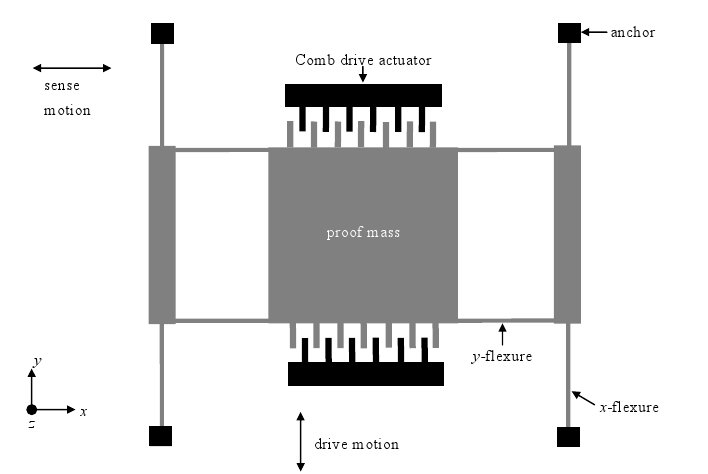
\includegraphics[width=0.8\linewidth]{Design}
\caption{The proposed design of a 2-DOF gyroscope.}
\label{fig:design}
\end{figure}

\begin{figure}[htb]
\centering
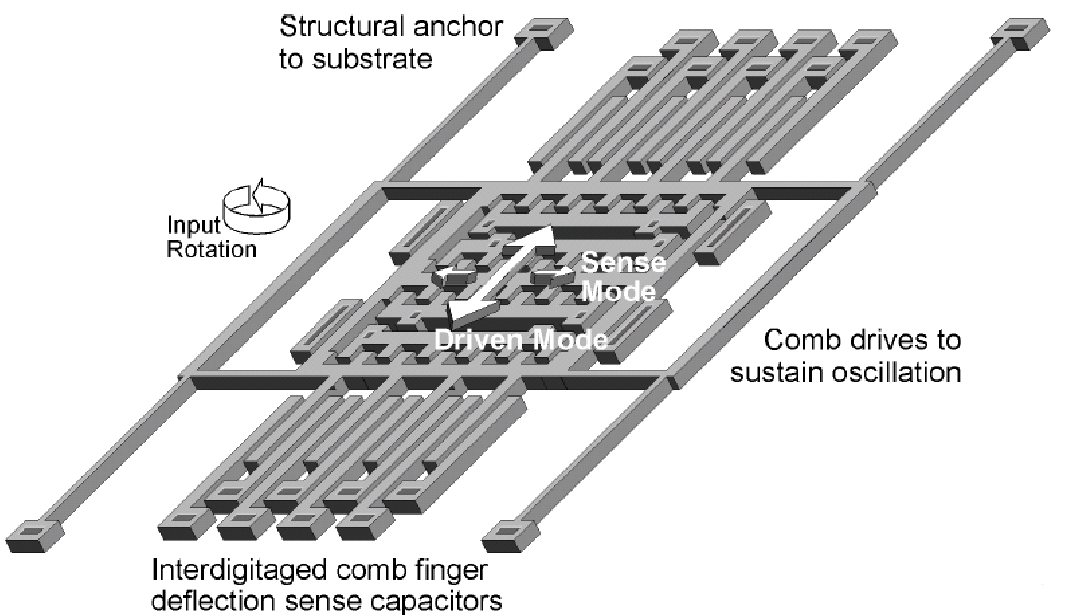
\includegraphics[width=0.8\linewidth]{capadesign}
\caption{A 2-DOF design with capacitive sensing. From \cite{Clark96}}
\label{fig:capadesign}
\end{figure}
\section{Derivations of device operation}
As we see from figure \ref{fig:design}, the device has beams acting as springs in both the drive and sense directions. We will consider these as cantilevers with a load applied to the end. Doing so yields the spring constant for a single beam expressed in equation \ref{eq:ksinglebeam} for a single beam. Expanding this into equation \ref{eq:kyorx} for the drive or sense directions, we arrive at an expression for the spring constant of the total system in both drive and sense directions by assuming that the 4 beams acting in each direction are identical. In these expressions E is the Youngs modulus and w, h and l the width, height and length of the beams in either the sensing or drive direction.

\begin{equation}
k_{single beam} = \dfrac{1}{4} \dfrac{E h w^3}{l^3}
\label{eq:ksinglebeam}
\end{equation}
\begin{equation}
k_{i,total} = 4 k_{single beam} = \dfrac{E h w_i^3}{l_i^3}
\label{eq:kyorx}
\end{equation}

With the proof mass oscillating in the drive direction one can describe the device as a 2-DOF vibratory system. The resulting equations of motions showed in equations \ref{eq:motiondrivedirection} and \ref{eq:motionsensedirection}. Here, $\omega_i$ is the resonance frequency in the i direction, $Q_i = \dfrac{m_i \omega_i}{b_i}$ is the quality factor, $b_i$ the damping factor, $\Omega$ the external rotation frequency and $F_d$ the electrostatic driving force. d and s subscripts denote sense (\textbf{x}) and drive (\textbf{y}) directions, respectively.

\begin{equation}
\ddot{y}+\dfrac{\omega_d}{Q_d} \dot{y} + \omega_d^2 y = \dfrac{F_d}{m} \sin(\omega_d t)
\label{eq:motiondrivedirection}
\end{equation}
\begin{equation}
\ddot{x} + \dfrac{\omega_s}{Q_s} \dot{x} + \omega^2 x + 2 \Omega \dot{y} = 0
\label{eq:motionsensedirection}
\end{equation}

Since gyroscopes generally are underdamped, it is reasonable to assume that the drive direction amplitude can be modelled as below.

\begin{equation}
y(t) = A_0 \sin(\omega_d t) = Q_d \dfrac{F_d}{k_y} \sin{\omega_d t}
\label{eq:yamplitudeast}
\end{equation}

By solving the system of differential equations\footnote{These expressions were found using Mathematica, and are identical to the once presented in %citation needed.
} 
above, we get the following expressions for the displacement and also a phase relative to the drive frequency.

\begin{equation}
x(t) = \dfrac{2 \Omega \cdot A_0 \omega_d}{\omega_s^2 \sqrt{\left(1-\left(\frac{\omega_d}{\omega_s}\right)^2\right)^2 + \left(\frac{\omega_d}{Q_s\cdot \omega_s}\right)}} \cdot \sin(\omega_d t - \varphi)
\label{eq:xoftraw}
\end{equation}
\begin{equation}
\varphi = \arctan \left(\dfrac{1}{Q_s \left(\frac{\omega_s}{\omega_d}- \frac{\omega_d}{\omega_s}\right)}\right)
\label{eq:phase}
\end{equation}

\begin{equation}
C(\omega) = \dfrac{1}{ \sqrt{\left(1-\left(\frac{\omega_d}{\omega_s}\right)^2\right)^2 + \left(\frac{\omega_d}{Q_s\cdot \omega_s}\right)}}
\label{eq:constant}
\end{equation}

\begin{equation}
\lvert X \rvert = \dfrac{2 \cdot \Omega \cdot A_0 \cdot C (\omega)}{\omega_s^2}
\label{eq:absolutedisplacementsense}
\end{equation}

In equation \ref{eq:bandwith} we see the bandwidth of a gyroscope at resonance, and by inserting into equation  \ref{eq:absolutedisplacementsense} we can analyse the bandwidth-sensitivity trade-off for the device. As seen in equation \ref{eq:bandwithsensitivitytradeoff}, the sensitivity of the device is heavily reliant on the bandwidth, in fact there is an inverse square dependence. This means that a narrow bandwidth is required. As the device is operated at ambient conditions, we will have to accept a loss in sensitivity as it is very difficult to achieve narrow bandwidths here.

\begin{equation}
B.W.= \dfrac{\omega_i}{Q_i}
\label{eq:bandwith}
\end{equation}
\begin{equation}
\dfrac{X}{\Omega}=\dfrac{2 \cdot A_0 \cdot C (\omega)}{\omega_s^2}=\dfrac{2 \cdot A_0 \cdot C (\omega)}{B.W.^2 \cdot Q_s^2}
\label{eq:bandwithsensitivitytradeoff}
\end{equation}

In addition, we need to consider the noise in the system. In this case, thermal noise will be present, caused by the Brownian force which can be expressed as in equation \ref{eq:BrownianForce}. By equating this with the Coriolis force, equation \ref{eq:Coriolisforce}, acting on the vibrating mass, we get an expression for the noise in the system, shown in equation \ref{eq:browniannoise}.

\begin{equation}
\lvert F_{Brownian}\rvert = \sqrt{4k_b T b_s B.W.} = \sqrt{\dfrac{4k_b T \omega_s m B.W.}{Q_s}}
\label{eq:BrownianForce}
\end{equation}

\begin{equation}
\lvert F_{Coriolis}\rvert = 2 m \lvert \dot{y} \rvert \Omega = 2 m \omega_d A_0 \Omega
\label{eq:Coriolisforce}
\end{equation}
\begin{equation}
2 m \omega_d A_0 \Omega = \sqrt{\dfrac{4k_b T \omega_s m B.W.}{Q_s}}
\label{eq:brownequcori}
\end{equation}
\begin{equation}
\dfrac{\Omega}{\sqrt{B.W.}} = \sqrt{\dfrac{k_b T \omega_s}{m Q_s A_0^2 \omega_d^2}}
\label{eq:browniannoise}
\end{equation}

Our last consideration is that of the driving force. In equations \ref{eq:combdrivecapacitance} and \ref{eq:capstoredenergy} we see the capacitance, $C$, and stored energy, $ U $, of a comb drive actuator, respectively. By differentiating the energy in the direction of movement of the actuator we get the expression for the force in equation \ref{eq:capforce}. In the following expressions, $\epsilon$ is the dielectric constant of the medium where the gyroscope operates, $l_0$ is the overlap length of the comb fingers, $h$ is the height of the fingers and, hence, the device, N is the total number of electrodes and $g_0$ is the nominal gap between the comb fingers and electrode as indicated on figure \ref{fig:design}.

\begin{equation}
C = \epsilon \dfrac{A_{overlap}}{g_0} = \epsilon \dfrac{2N \cdot (l_0 +y) h  }{g_0}
\label{eq:combdrivecapacitance}
\end{equation}
\begin{equation}
U = \dfrac{1}{2} C V^2
\label{eq:capstoredenergy}
\end{equation}
\begin{equation}
F = -\nabla U = - \dfrac{1}{2} \dfrac{\delta C}{\delta y} V^2 = -\dfrac{\epsilon \cdot N  \cdot h}{g_0} V^2
\label{eq:capforce}
\end{equation}

By applying different voltages, $V_1 = V_0 + v(t)$ and $V_2 = V_0 - v(t)$, to the top and bottom electrodes one induces an effective force acting on the mass\supercite{Chang12}. Here $V_0$ is a DC bias and $v(t)$ an applied AC bias.

\begin{equation}
F_{drive} = F_{top} - F_{bottom} = -4\dfrac{\epsilon \cdot \frac{N}{2}  \cdot h}{g_0} V_o v(t)
\end{equation} 



\section{Numerical Analysis}
To approach a functioning device we will now apply some of the design constraints to the derived expressions above to try to optimise device operation.In table \ref{tab:designconstraints}, we see a summary of the design constraints that will be used below.

\begin{table}[htbp]
\caption{Table showing some of the design constraints}
\centering
\begin{tabular}{l|r}
\toprule
Maximum design area (mm) & {2 x 2} \\ 
Min dimensions of proof mass ($\mu$m) & {500 x 500} \\ 
Min beam width ($\mu$m) & 2 \\ 
Max beam deflection (\%) & 2 \\
Thickness of structure ($\mu$m) & 6 \\ 
Max flexure length($\mu$m) & 500 \\ 
Min electrode gap ($\mu$m) & 0.5 \\ 
Vertical gap between structure and substrate ($\mu$m) & 2 \\ \bottomrule
\end{tabular}
\label{tab:designconstraints}
\end{table}

\subsection{Flexure design}
From equation \ref{eq:browniannoise}, it is evident that the Brownian noise in the system is highly dependent on the amplitude of the driving vibrations. As the beam deflection is limited to 2 \% of the beam length it is therefore reasonable to chose the longest possible beams of 500 $\mu$m. Furthermore, we see from equation \ref{eq:yamplitudeast} that the amplitude is inversely proportional to the mechanical spring constant in the drive direction, we therefore wish to minimise this quantity by choosing the minimum beam width of 2 $\mu$m with the thickness of the structure fixed at 6 $\mu$m and Youngs modulus of silicon of 130 GPa assuming that the bending is in the [100]-direction \supercite{Bhushan97}.

\begin{equation}
k_d = \dfrac{E h w_d^3}{l_d^3}= 0.05 Nm^{-1}
\label{eq:drivespringconstant}
\end{equation}

Equation \ref{eq:drivespringconstant} along with the given resonance frequency in the drive direction makes it possible to calculate the proof mass as in equation \ref{eq:springconsttomass}.

\begin{equation}
\omega_d = \sqrt{\dfrac{k_d}{m}} \rightarrow m = \dfrac{k_d}{\omega_d^2} = 1.26 \cdot 10^{-11} kg
\label{eq:springconsttomass}
\end{equation}

If we assume a quadratic, seen from the top, proof mass we can find the dimensions as seen in  equation \ref{eq:flexdimensionsfirst} below. Here, $\rho_Si$ is the density of silicon, $V$ the volume of the mass and $l_m$ the mass dimensions in the xy-plane of the device.

\begin{equation}
\rho_Si = \dfrac{m}{V} = \dfrac{m}{l_m^2 h} \leftrightarrow l_m = \sqrt{\dfrac{m}{\rho_Si h}} = 30 \mu m
\label{eq:flexdimensionsfirst}
\end{equation}

As we see this result is far below the minimum mass dimensions and we will have to iterate our results to find suitable flexure dimensions. Furthermore, we will chose a rectangular proof mass with width 510 $\mu$m and the length maximised so that to mount the most electrodes possible on it. In table \ref{tab:1stiteration}, values for the 1st iteration are put.

\begin{table}[htbp]
\caption{Table showing iterated dimensions}
\centering
\begin{tabular}{lllllll}
\toprule
$w_d [\mu m]$ & $l_d [\mu m]$ & $k_d$[N/m] & m [$\mu g$] & $w_{mass} [\mu g]$ & $l_{mass} [\mu m]$ & $A_0 [\mu m]$ \\ \midrule
\multicolumn{1}{r}{5} & \multicolumn{1}{r}{130} & \multicolumn{1}{r}{44.38} & \multicolumn{1}{r}{11.2} & \multicolumn{1}{r}{510} & \multicolumn{1}{r}{1530} & \multicolumn{1}{r}{2.6} \\ \bottomrule
\end{tabular}
\label{tab:1stiteration}
\end{table}

By assuming that the support structure has negligible weight we now can calculate the flexure dimensions in the sense direction. To minimize the flexure length, $l_s$, we chose the minimum flexure width of 2 $\mu$m.

\begin{equation}
l_s = \sqrt[3]{\dfrac{E t w_s^3}{m \omega^2} } =
\label{eq:senselength}
\end{equation}

We have chosen a resonance frequency in the sense direction that is slightly off-set from the one in the drive direction. This is done to increase the gyroscope's robustness, in fact an off-set like this makes it possible to control the bandwidth in a dynamic response. If the two resonance frequencies are matched there is a danger that the sensor will become insensitive to changes in the rotational frequency.

\subsection{Actuator force and Damping}

We still have to consider the driving force and optimise the electrode arrangement. To do this we will also have to consider the damping, and, hence the Q-factor, of the system, specially in the drive direction.

We will assume that the damping is dominated by Couette flow between the proof mass and the substrate. The equation for this is shown below (\ref{eq:drivedamping}) and using the data from table \ref{tab:1stiteration} and the separation of the mass and substrate of 2 $\mu$m along with the viscosity of air at room temperature, $\eta$, of 1.8 kg/m$\cdot$ s. This allows us to estimate the quality factor in the drive direction as shown in equation \ref{eq:Qfactordrivecalc1}

\begin{equation}
b_d = \dfrac{\eta A_{mass}}{h}= \dfrac{\eta l_d w_d}{h} = 7.03\cdot 10^{-6} kg \cdot s^{-1}
\label{eq:drivedamping}
\end{equation}

\begin{equation}
Q_d = \dfrac{m_d \omega_d}{b_d} = 100.53
\label{eq:Qfactordrivecalc1}
\end{equation}

To improve on the results above, we will now consider the damping due to the comb-drive fingers moving in and out of the gap. Once again we will assume that Couette flow is dominant and that we want to maximise the force and therefore minimize the electrode gap, $g_0$. The length of the comb fingers is set to 5.3 $\mu$m to allow for the maximum amplitude of the vibrations and gaps of 0.5 $\mu$m to avoid short circuiting the system. The width of the fingers is set at 2 $\mu$m to maximize the amount of fingers one can place on each side of the proof mass.

\begin{equation}
F_d = A_0 \dfrac{k_d}{Q_d} = 1.15 \mu N
\label{eq:driveforce1stapprox}
\end{equation}

\begin{equation}
N/2 = \dfrac{F_d g_0}{4 \epsilon h V_{AC} V_{DC} } = 270
\label{eq:fingers1st}
\end{equation}

\begin{equation}
N/2_{max}= \dfrac{l_{mass}}{l_{electrode}} = 306
\label{eq:fingersmax}
\end{equation}

As we see from equations \ref{eq:fingers1st} and \ref{eq:fingersmax}, there is a need for 270 fingers each side of the proof mass to achieve the force required and that this is possible to fit in on the side of the proof mass. However, damping from these fingers becomes important and we will need to consider this in order to find a more accurate expression for the damping. Assuming that damping of the fingers is dominated by Couette flow we arrive at equation \ref{eq:dampingwithcomb} for the total damping. Note here that the number of fingers now will both affect damping and the maximum driving force, equation \ref{eq:capforce}. We will assume that the overlap along the drive direction is equal to two times the amplitude, $l_0 = 2A_0 = 5.2 \mu m$, to allow the proof mass to complete it's cycles.

\begin{equation}
b_{tot} = \eta \dfrac{A_mass}{h} + \eta \dfrac{4 \frac{N}{2} t l_0}{g_0}
\label{eq:dampingwithcomb}
\end{equation}

The damping factor now depends on the number of combs which will change with a changing quality factor. We will therefore need to enter this into the equation for the quality factor, $Q_d$, to calculate the optimal number of comb fingers.

\begin{equation}
N/2 = \dfrac{g_0 A_0 k_d \eta A_{mass}}{ht(4 \epsilon_0 V_DC V_AC \omega_d m - A_0 k_d \eta 4 A_0)} = 296
\label{eq:comfingers2ndit}
\end{equation}

The number of fingers calculated above still is below the maximum per half. To minimise the power consumption we could optimize the device set-up with regards to the voltages used, but as we are pretty close to the maximum value the direct current could not be inferior to 9.97 V, meaning one could only possibly save 3 \% of the total power consumption. In the following calculation we have therefore used the number of comb drives as calculated above.

Below, we calculate the new Q$_d$:

\begin{equation}
Q_d = \dfrac{\omega_d m}{\eta \left(\frac{4N A_0t}{g_0} + \frac{A_{mass}}{h}\right)}= 84.5
\label{eq:qualityfactorit}
\end{equation}

So far, we have considered the comb fingers to be massless. To adjust our calculations we will now consider the weight of the comb fingers with a length of 5.3 $\mu$m and a width of 2 $\mu$m. The additional mass is shown in equation \ref{eq:masscombfingers}, which leads us to recalculate the width of the mass in equation \ref{eq:widthfinal}.

\begin{equation}
m_{comb fingers} = N w_{finger} t l_finger \rho_Si = 9.04 \cdot 10^{-11} kg
\label{eq:masscombfingers}
\end{equation}

\begin{equation}
w_mass = \dfrac{m_{tot} - m_fingers}{\rho_{Si} t l_{mass}} = 506 \mu m
\label{eq:widthfinal}
\end{equation}

Putting the new dimensions into the equations for number of fingers and quality factor above changes neither and we will therefore stick with these dimensions for the next parts.

\subsection{Sense mode calculations and Brownian noise}
We will now look at the calculations in the sense mode. First, let us look at the damping factor. As we use an optical measuring system, there is no need for additional electrodes and we only have to consider the damping due to the proof mass and comb fingers. The damping is dominated by two effects, namely Couette flow between the proof mass and substrate and squeeze film flow between the comb fingers and fixed electrodes. In equation \ref{eq:dampingsense}, we see an expression for the damping in the sense direction. We assume that the average overlap between the fingers and fixed electrodes is equal to the amplitude of vibration, $A_0$.

\begin{equation}
b_s = \dfrac{\eta A_{mass}}{h} + \dfrac{2N \cdot 96 \cdot \eta\cdot t \cdot l_o^3}{\pi^4 \cdot g_0^3}= 2.47 \cdot 10^-5
\label{eq:dampingsense}
\end{equation}

\begin{equation}
Q_s = \dfrac{m \omega_s}{b_s} = 31
\end{equation}

We now can consider the thermal noise in the system at room temperature by using equation \ref{eq:browniannoise}.

\begin{equation}
\dfrac{\Omega_z}{\sqrt{B.W.}} = 1.74\cdot 10^{-4} rad/s/\sqrt{Hz}= 0.59 ^\circ /min/\sqrt{Hz}
\label{eq:browniannoiseactual}
\end{equation}

This value is well below the limit of 1 deg/min/$\sqrt{Hz}$ and we may therefore use this design.

Using equation \ref{eq:absolutedisplacementsense} we can calculate the displacement in the sense direction. We will assume a constant rotation about the z-axis of 1 deg/s when calculating this displacement.

\begin{equation}
\lvert X \rvert = \dfrac{2 \cdot 1 ^\circ /s \frac{2 \pi}{360^\circ} \cdot 2.6\mu m \cdot (2\pi \cdot kHz)}{(2\pi\cdot 11 kHz)^2\sqrt{(1-\frac{10}{11})^2 + (\frac{10}{11\cdot 31})^2}} = 2.86 pm
\label{eq:sensedisplacement}
\end{equation}

This displacement is very small and, as we see in equation \ref{eq:displacementcomp} below, if we compare it to the driven displacement it becomes even smaller.

\begin{equation}
\dfrac{\lvert X \rvert}{\lvert Y \rvert}/\Omega_z = 1.1\cdot 10^{-6} /^\circ/s
\label{eq:displacementcomp}
\end{equation}

The consequence of this finding is that the device read out is very vulnerable to coupling of the drive and Coriolis induced motions. For the device fabrication this has the implication that one needs to have an entirely decoupled motion in the sense and drive directions and, hence, no fabrication imperfections can be tolerated. If this is not done, the coupling would induce noise that easily could overwhelm the induced oscillations.

\subsection{Additional objectives to real gyroscopes}
Real life gyroscopes would probably be subjected to less strict spatial demands, but would have to serve additional objectives. For instance, the sensing of the displacement would have to be very sophisticated and would probably merit a large capacitive area sensing electrodes as shown in figure \ref{fig:capadesign} and more sensitive gyroscopes could be optimized to sense the rate of change of the rotation as well as a constant rotation rate. Furthermore, the device is required to operate for long periods of time with constant device performance.

These requirements once again states that imperfections in the fabrication process has to be avoided. In fact, inaccuracies in the fabrication process like over-etching or inaccurate lithography processes could potentially cause so big fluctuations in device performance that the device would be rendered non-operational.

\section{Possible device improvements}
In this section we will briefly look at which design choices one could possibly make to improve its' overall performance. The easiest way of improving the device would be to make the device more symmetric and reduce the coupling of the drive and sense modes. To do this, one would have to increase the power input which would be undesirable in, for instance, mobile applications. 

More impertinent is the fact that most of our considerations so far have been very crude, both when considering the damping and the electrostatics. Numerical simulations and modelling would offer great improvement to the actual performance. More accurate simulations could also help identify where in the fabrication process the errors are mostly affecting performance.

Lastly, an improvement to the 2-DOF design could be to introduce more degrees of freedom by adding a passive proof mass amplifying the driven mass' movement. This would relax the need for mode matching allowing the drive and sense mode to be tuned separately. It is also possible to expand the device to sense rotation about several axis on one chip which could potentially greatly improve the performance of the gyroscope\cite{An99}.




\end{spacing}
\printbibliography
\end{document}
